\documentclass[aspectratio=169]{beamer}

\usepackage{amsmath, amssymb}
\usepackage{bm}
\usepackage{graphicx}


\usepackage{appendixnumberbeamer}


\usetheme[
        %titleformat = allsmallcaps,
        numbering = fraction, 
        progressbar = head, 
        block = fill 
        %background = dark
        ]{metropolis}
\usecolortheme{spruce}
\usefonttheme[onlymath]{serif}

\title{\Large Coexistence on the Boundary of Communities}
\subtitle{\small Dispersal in Continuum Could Lead to the Coexistence of Unstable Species Combination}
\date{\today}
\author{Chang Longxiao, longxiao.chang@campus.lmu.de}
\institute{EES, Ludwig-Maximilian Universit\"{a}t M\"{u}nchen}

\begin{document}

    \maketitle

    \begin{frame}{Content}
        \tableofcontents
    \end{frame}

    \section{Introduction}

    \begin{frame}
        The fundamental model is generalized Lotka-Volterra model:
        \begin{equation*}
            \frac{\mathrm{d}N_i}{\mathrm{d}t}
            = N_i \left( r_i - N_i - \sum_{j\neq i} A_{i,j} N_j \right)
        \end{equation*}
        A general form to write it is:
        \begin{equation}
            \frac{\mathrm{d}N_i}{\mathrm{d}t}
            = N_i \left( r_i - \sum_{j} A_{i,j} N_j \right)
        \end{equation}

        As well as in matrix form
        \begin{equation*}
            \frac{\mathrm{d}\bm{N}}{\mathrm{d}t}
            = \bm{N} \left( \bm{r} - A \bm{N} \right)
        \end{equation*}
    \end{frame}

    \begin{frame}
        \begin{figure}
            \centering
            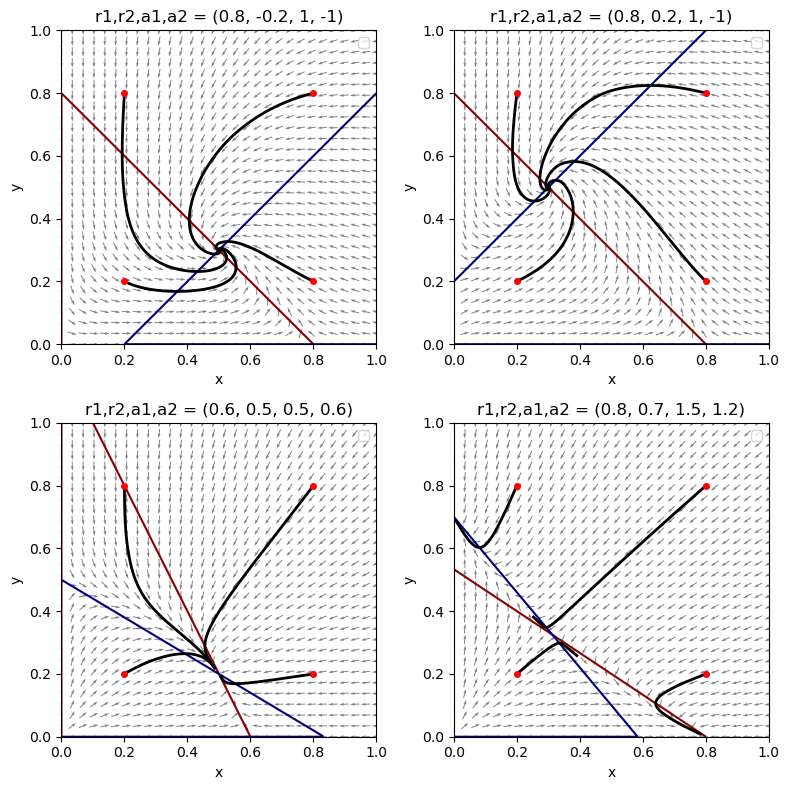
\includegraphics[scale = 0.4]{../../figure/competing_bistable.png}
        \end{figure}
    \end{frame}

    \section{Basic Idea}

    \begin{frame}
        \begin{columns}
            \column{0.55 \textwidth}
            When two species cannot coexist in GLV (for example because of competition), they could still coexist in a continuous space. 
            
            A simple example is a three patches model. Considering species 1 occupied the first patch and species occupied the third, both of hem could invade patch 2, but no individual could escape, in this case, both of them could coexist in the middle.

            This also holds in continuous space (homogenous enviroment), as shown at the right.
            \column{0.45\textwidth}
            \begin{figure}
                \centering
                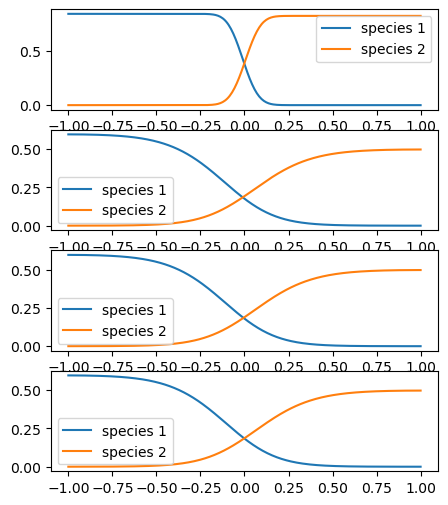
\includegraphics[scale = 0.6]{../../figure/strong_comp.png}
            \end{figure}
        \end{columns}
        
    \end{frame}

    \begin{frame}
        As a result, we would also guess that not only two species, but more species could coexist even the total community is not stable. That is, considering the community could be divided into two sub-communities that are stable, if both of them cannot invade the other, all the species will coexist in the region where the two communities meet.
    \end{frame}

    \section{Model}

    \begin{frame}
        The basic framework is a \textbf{Diffusion-Reaction Model}, where diffusion term is a second ordered partial differentiation, while reaction term is just GLV.
        \begin{equation}
            \frac{\mathrm{d}N_i}{\mathrm{d}t}
            = D_{i}\frac{\partial^2 N}{\partial x^2} +
            N_i \left( r_i - \sum_{j} A_{i,j} N_j \right)
        \end{equation}
        In short:
        \begin{equation*}
            \partial_t N = D_i \nabla^2_x N + N (r - AN)
        \end{equation*}
    \end{frame}

    \section{The simplest case}

    \subsection{One species}

    \begin{frame}{Fischer-KPP Equation}
        \begin{equation}
            \frac{\partial N}{\partial t} = D\frac{\partial^2 N}{\partial x^2} +  N(r-N)
        \end{equation}
        By rescaling:
        \begin{equation*}
            \partial_t N = \nabla^2_x N +  rN(1-N)
        \end{equation*}
    \end{frame}

    \begin{frame}{Allen-Cahn equation}
        \begin{equation}
            \partial_t N = \nabla^2_x N +  rN - aN^3
        \end{equation}

        \begin{equation*}
            N(x,t) = \tanh\left( \frac{x-x_0}{\sqrt{2}} \right)
        \end{equation*}
    \end{frame}

    \subsection{Two speices}

    \begin{frame}{Two Species Model}
        \begin{equation}
            \begin{cases}
                \frac{\partial N_1}{\partial t}
                = D_{1}\frac{\partial^2 N_1}{\partial x^2} +
                N_1 \left( r_1 - A_{1,1} N_1 - A_{1,2} N_2 \right)\\
                \frac{\partial N_2}{\partial t}
                = D_{2}\frac{\partial^2 N_2}{\partial x^2} +
                N_2 \left( r_2 - A_{2,2} N_2 - A_{2,1} N_1 \right)
            \end{cases}
        \end{equation}
        \begin{equation*}
            \begin{cases}
                \partial_t N_1
                = \nabla^2_x N_1 +
                N_1 \left( 1 - N_1 - k N_2 \right)\\
                \partial_t N_2
                = d \nabla^2 N_2 +
                r N_2 \left( 1 - N_2 - h N_1 \right)
            \end{cases}
        \end{equation*}
    \end{frame}

    \begin{frame}{Symmetrical Condition}
        \begin{equation*}
            \begin{cases}
                \partial_t N_1
                = d \nabla^2_x N_1 +
                r N_1 \left( 1 - a N_1 - b N_2 \right)\\
                \partial_t N_2
                = d \nabla^2 N_2 +
                r N_2 \left( 1 - a N_2 - b N_1 \right)
            \end{cases}
        \end{equation*}
         Could be approximated to Allen-Cahn equation
    \end{frame}

    \begin{frame}
        
    \end{frame}

    \begin{frame}{Simulations}
        \begin{columns}
            \column{0.5\textwidth}
            \begin{equation*}
            \begin{cases}
                \partial_t N_1
                = (1+a) \nabla^2_x N_1 +
                1 N_1 \left( 1 - N_1 - 1.5N_2 \right)\\
                \partial_t N_2
                = 1\nabla^2 N_2 +
                (1-b) N_2 \left( 1 -  N_2 - 1.5 N_1 \right)
            \end{cases}
        \end{equation*}
        \column{0.5\textwidth}
        \begin{figure}
            \centering
            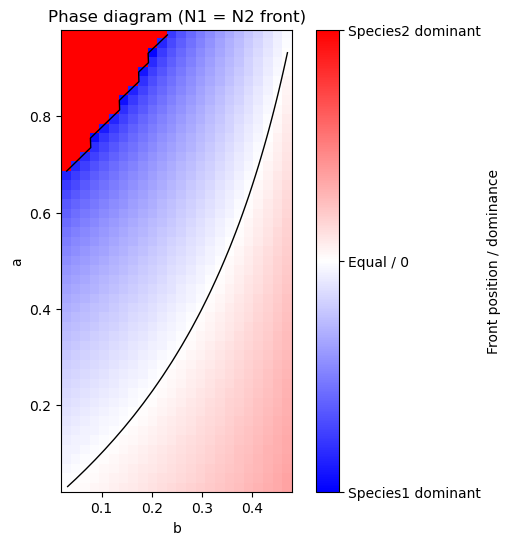
\includegraphics[scale = 0.5]{../../figure/balance_rD_clear.png}
        \end{figure}
        \end{columns}
    \end{frame}

    \begin{frame}
        \begin{figure}
            \centering
            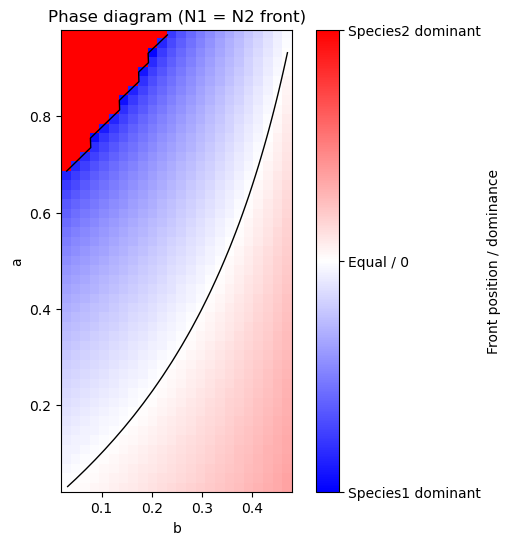
\includegraphics[scale = 0.6]{../../figure/balance_rD_clear.png}
        \end{figure}
    \end{frame}

    \begin{frame}{Simulations}
        \begin{columns}
            \column{0.5\textwidth}
            \begin{equation*}
            \begin{cases}
                \partial_t N_1
                = \nabla^2_x N_1 +
                1 N_1 \left( 1 - N_1 - (1+a) N_2 \right)\\
                \partial_t N_2
                = 1\nabla^2 N_2 +
                (1-b) N_2 \left( 1 -  N_2 - (1+a) N_1 \right)
            \end{cases}
        \end{equation*}
        \column{0.5\textwidth}
        \begin{figure}
            \centering
            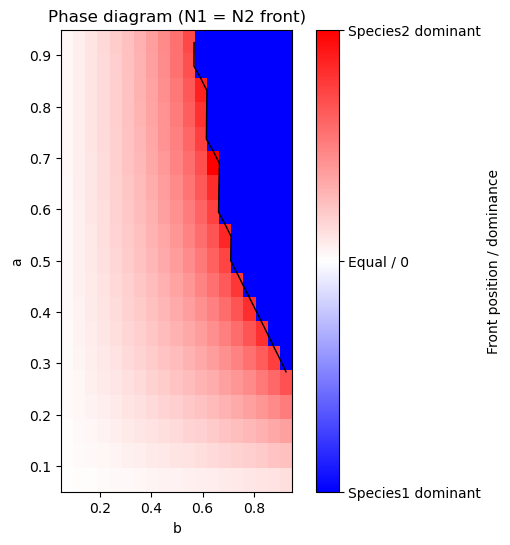
\includegraphics[scale = 0.5]{../../figure/balance_rk.png}
        \end{figure}
        \end{columns}
    \end{frame}

\end{document}